\section{Results}

\subsection{Basic Results}

The first example we will show is 3 UAS estimating a wind gradient with an $a = 1.5$ and $b = 10$.
The wind direction is assumed to be in the [1, 1, 0] inertial direction.
These UAS are initalized and commanded to follow a series of lines 25 feet apart and off the ground.
Thus, there is a UAS flying at 25 m, 50 m, and 75 m from the ground.
The aircraft will be simulated for 50 seconds, with a speed of 18 m/s and an EKF update rate of 1 Hz.
The trajectories of the aircraft can be seen in Figure~\ref{fig:uas_traj_three}.

\begin{figure}[h]
    \centering
    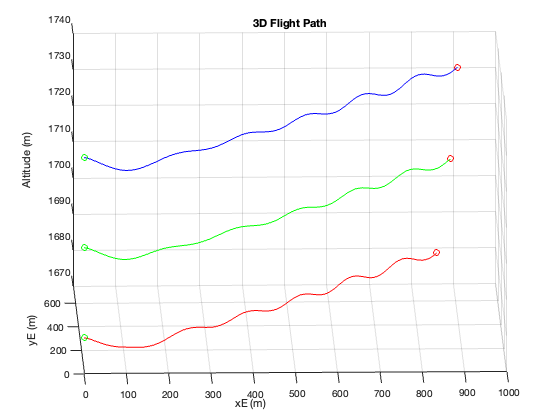
\includegraphics[width=0.5\textwidth]{images/uas_traj_3.png}
    \caption{Trajectories of 3 UAS spread apart by 25 m guidance lines. Flying in a wind gradient with $a = 1.5$ and $b = 10$ in the [1, 1, 0] inertial direction.}
    \label{fig:uas_traj_three}
\end{figure}

As you can see from the figure, the UAS are able to accurately follow their straight, level, guidance lines with only some oscillations.

Now, looking at the estimated wind gradient figures we can see the progression difference between 2.5 seconds vs 7 seconds vs 15 seconds into the simulation.
These can be seen in Figures~\ref{fig:uas_traj_three_25}, ~\ref{fig:uas_traj_three_75}, and ~\ref{fig:uas_traj_three_15}.

\begin{figure}[h]
    \centering
    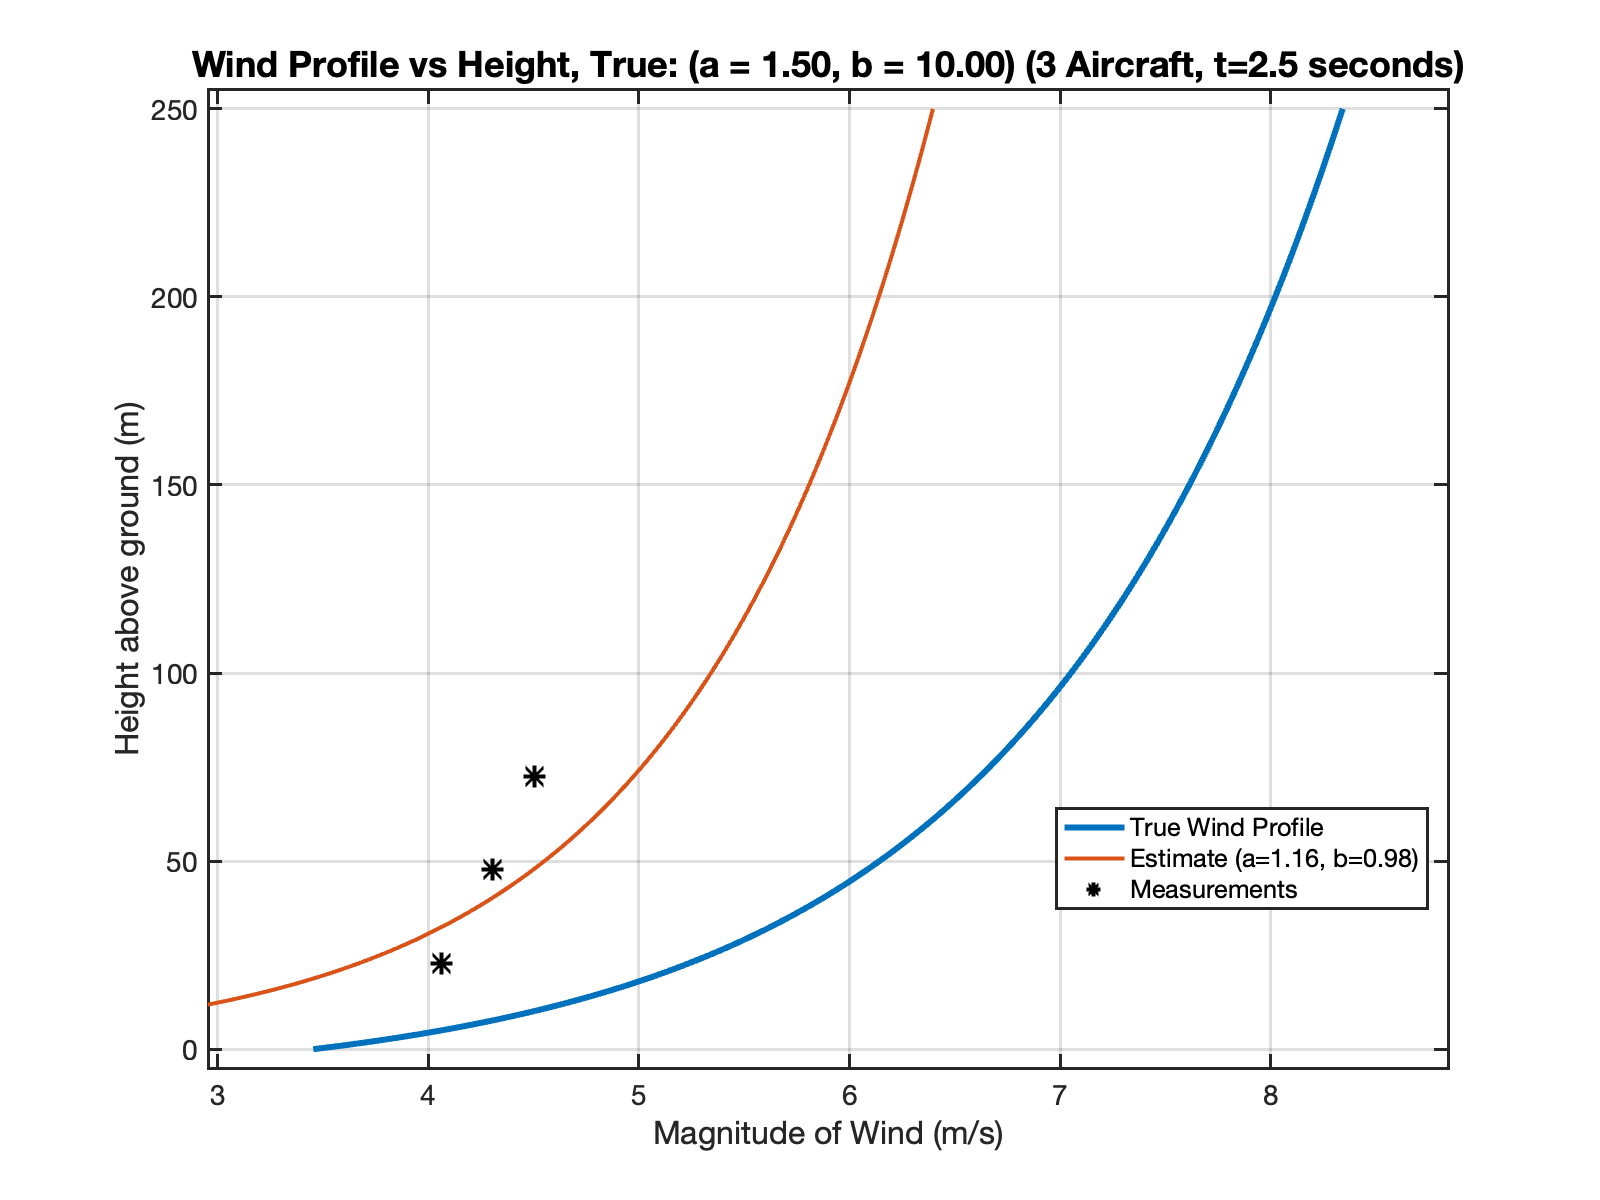
\includegraphics[width=0.5\textwidth]{images/3_uas_2.5_sec.png}
    \caption{3 UAS, estimated wind gradient after 2.5 seconds into the simulation.}
    \label{fig:uas_traj_three_25}
\end{figure}

\begin{figure}[h]
    \centering
    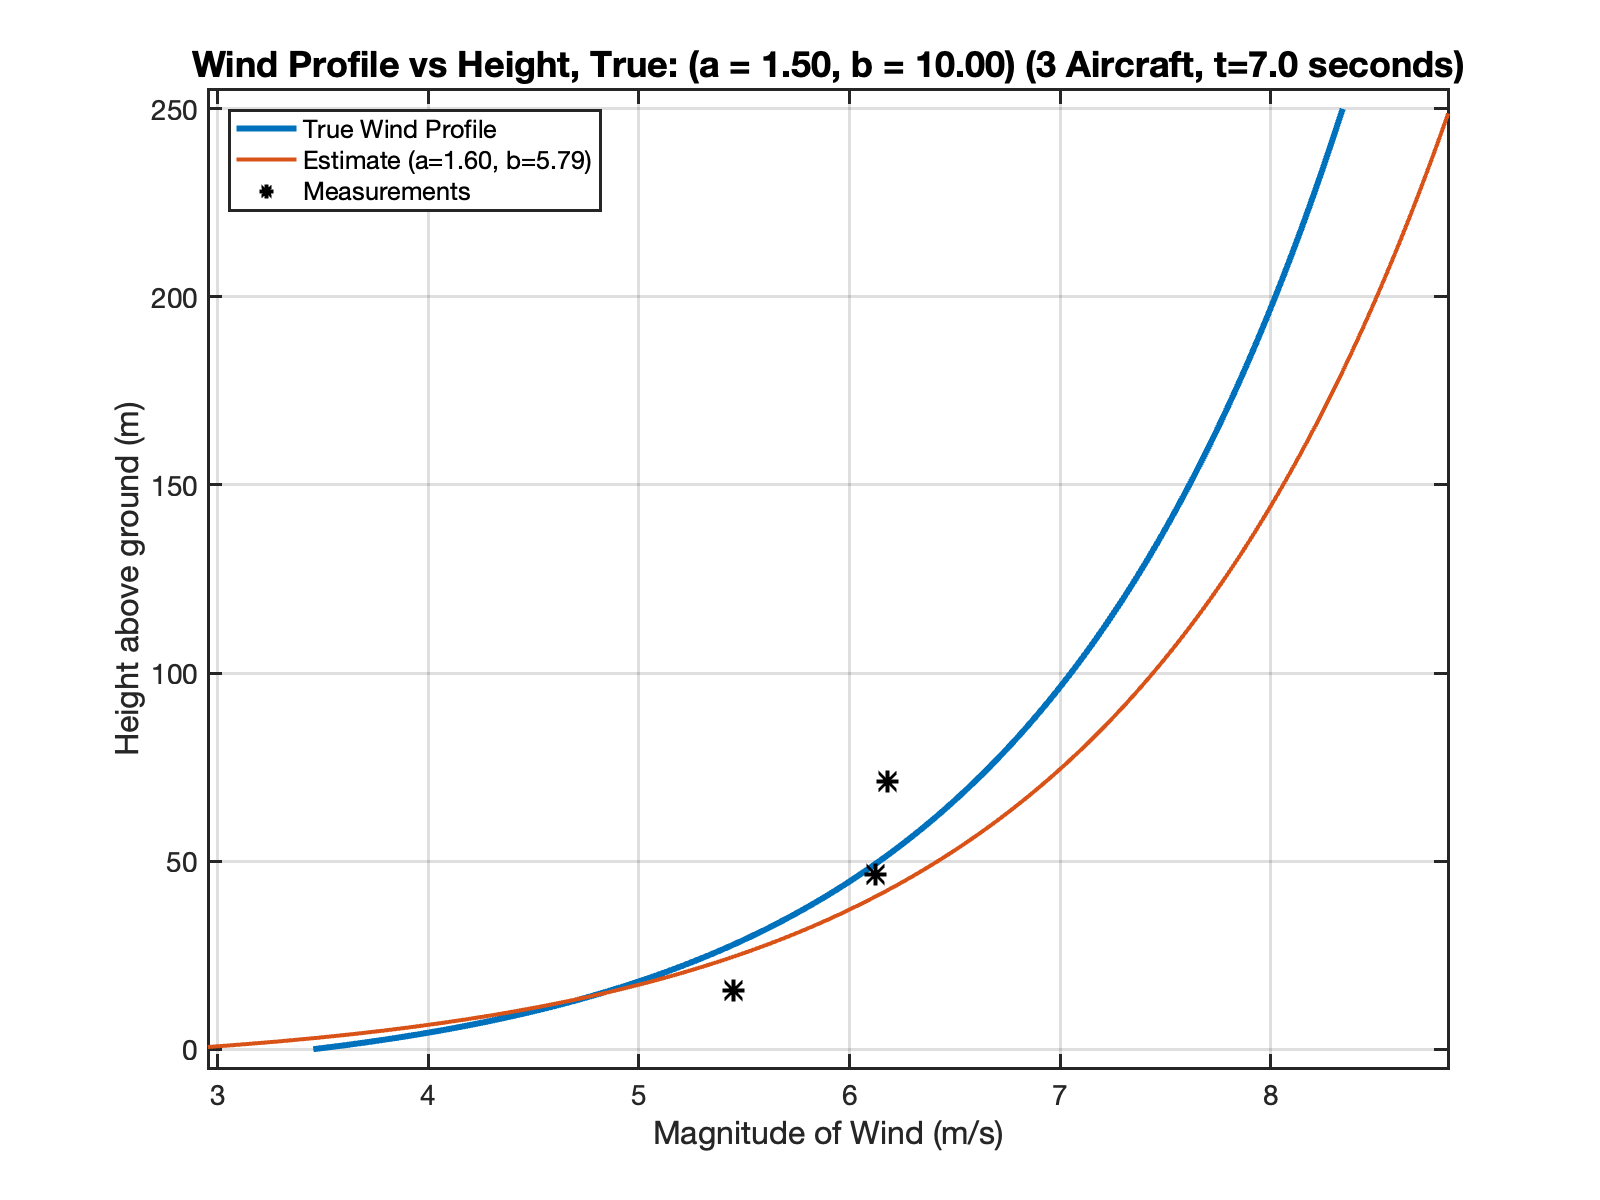
\includegraphics[width=0.5\textwidth]{images/3_uas_7_sec.png}
    \caption{3 UAS, estimated wind gradient after 7 seconds into the simulation.}
    \label{fig:uas_traj_three_75}
\end{figure}

\begin{figure}[h]
    \centering
    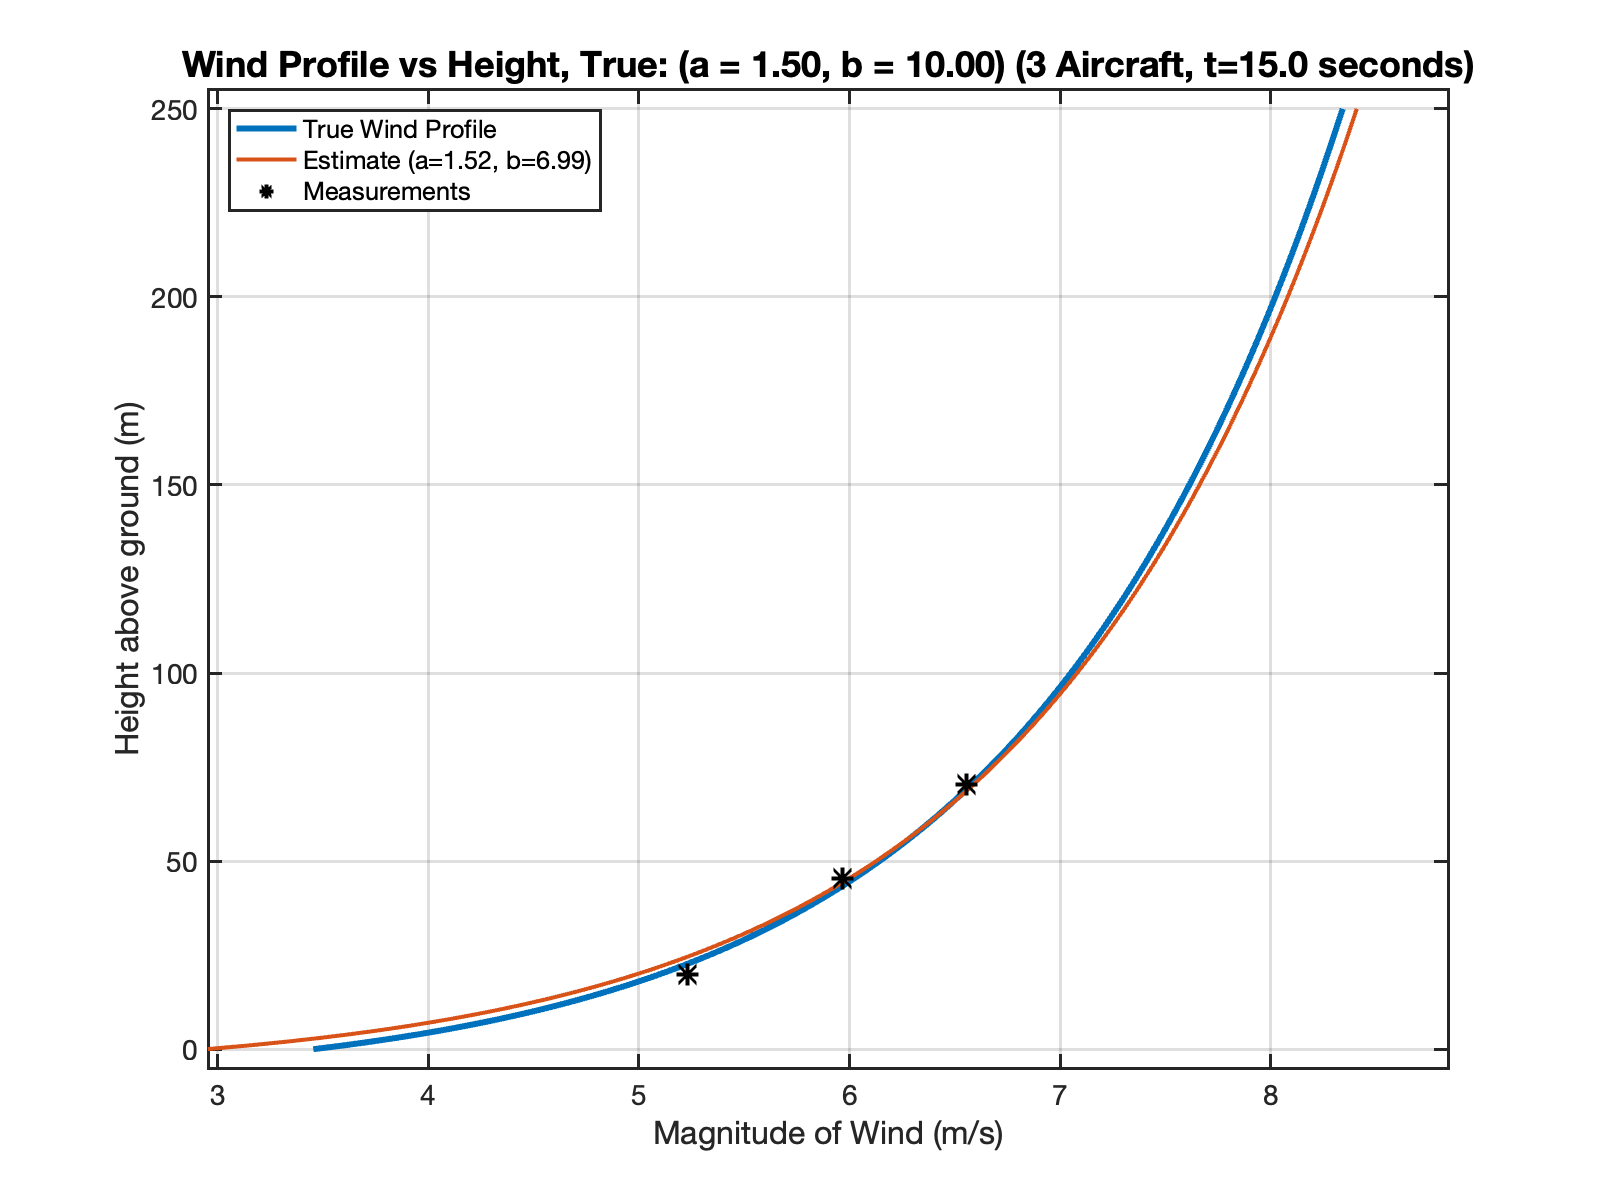
\includegraphics[width=0.5\textwidth]{images/3_uas_15_sec.png}
    \caption{3 UAS, estimated wind gradient after 15 seconds into the simulation.}
    \label{fig:uas_traj_three_15}
\end{figure}

The blue line represents the true wind gradient field that is impacting the UAS during flight.
The red line represents the current time estimate of the wind gradient field, using the $a$ and $b$ values specified in the legend.
The scatter points represent the current time estimate of a UAS position and the wind magnitude at that position.

Theres three interesting things to observe that are occuring as time progresses.
First, the UAS are able to gain steady altitude flight; correctly following their guidance lines. 
You can see in Figure~\ref{fig:uas_traj_three} that the UAS flight paths have the biggest oscillations at the start of the simulation before they steady out.
Second, as time progresses, each UAS is able to estimate its own wind field more accurately.
The difference between time 2.5 and 7 seconds shows how the scatter dots representing the UAS measured height and wind magnitude is much more accurate in the wind (x-axis) measurement.
Third, as follows from each UAS being able to accurately estimate their own wind magnitude, the overall estimated relationship of the wind gradient field begins to converge to the true wind gradient field.

This result is really a cumulative sum of all three relationships. As the UAS's autopilot is able to level out to the guidance line commanded, 
the wind measurements become more steady as the UAS is not traversing the gradient (as touched on in the \textit{Adjusting the EKF} section).
This allows the EKF to more accurately estimate the individual UAS wind measurements at that commanded height. 
With a continous stream of accurate individual wind measurements, the stochastic gradient descent algorithm can accurately converge to the correct $a$ and $b$ values that describe the true wind gradient field.
Thus, all 3 systems: the UAS autopilot, the wind EKF, and the central gradient estimator work together to accurately estimate the wind gradient field.

A video showing the full simulation over 50 seconds can be seen in the link at the top of the paper.

\subsection{Single UAS Edge Case}

An interesting edge case to consider is if this algorithm is able to successfully estimate the wind gradient with only a single UAS.
The series of results showing the same wind gradient as above, but, now with only a single UAS commanded to fly at 25 m above the ground can be seen in the Figures~\ref{fig:uas_traj_one_5} and~\ref{fig:uas_traj_one_15}.

\begin{figure}[h]
    \centering
    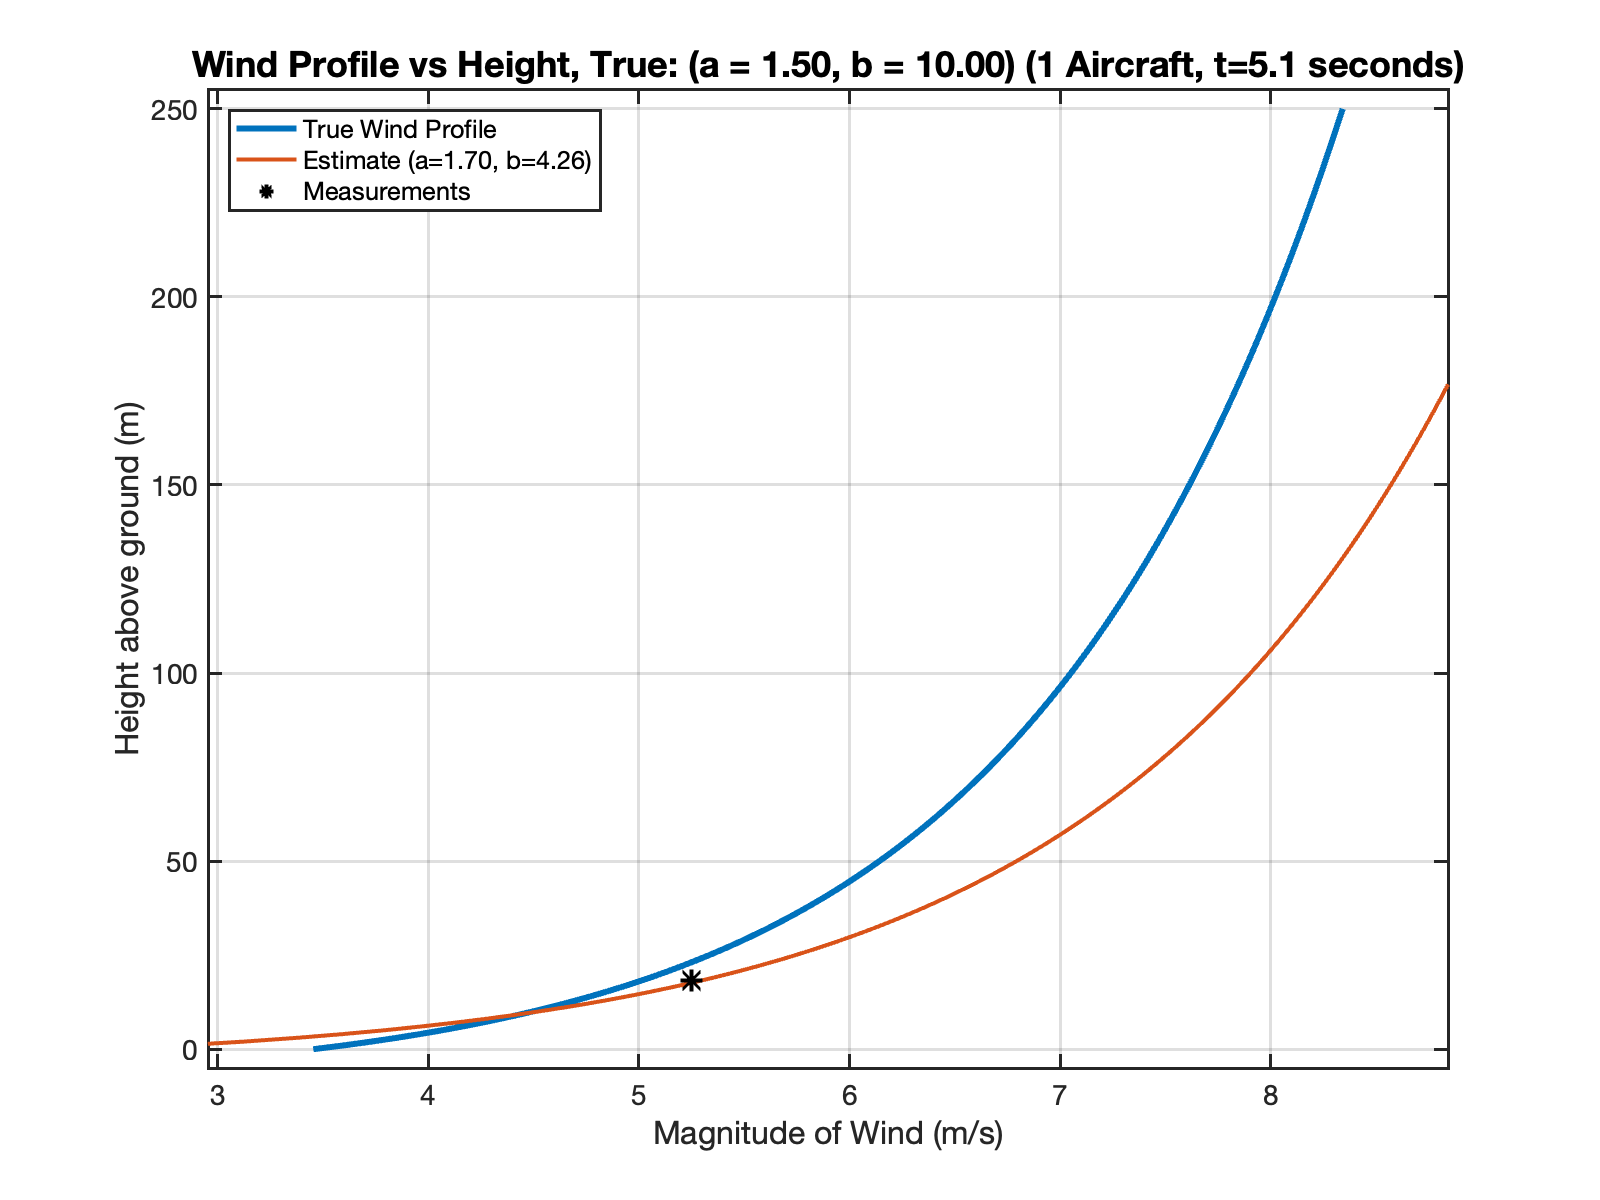
\includegraphics[width=0.5\textwidth]{images/single_5_sec.png}
    \caption{1 UAS, estimated wind gradient after 5 seconds into the simulation.}
    \label{fig:uas_traj_one_5}
\end{figure}

\begin{figure}[h]
    \centering
    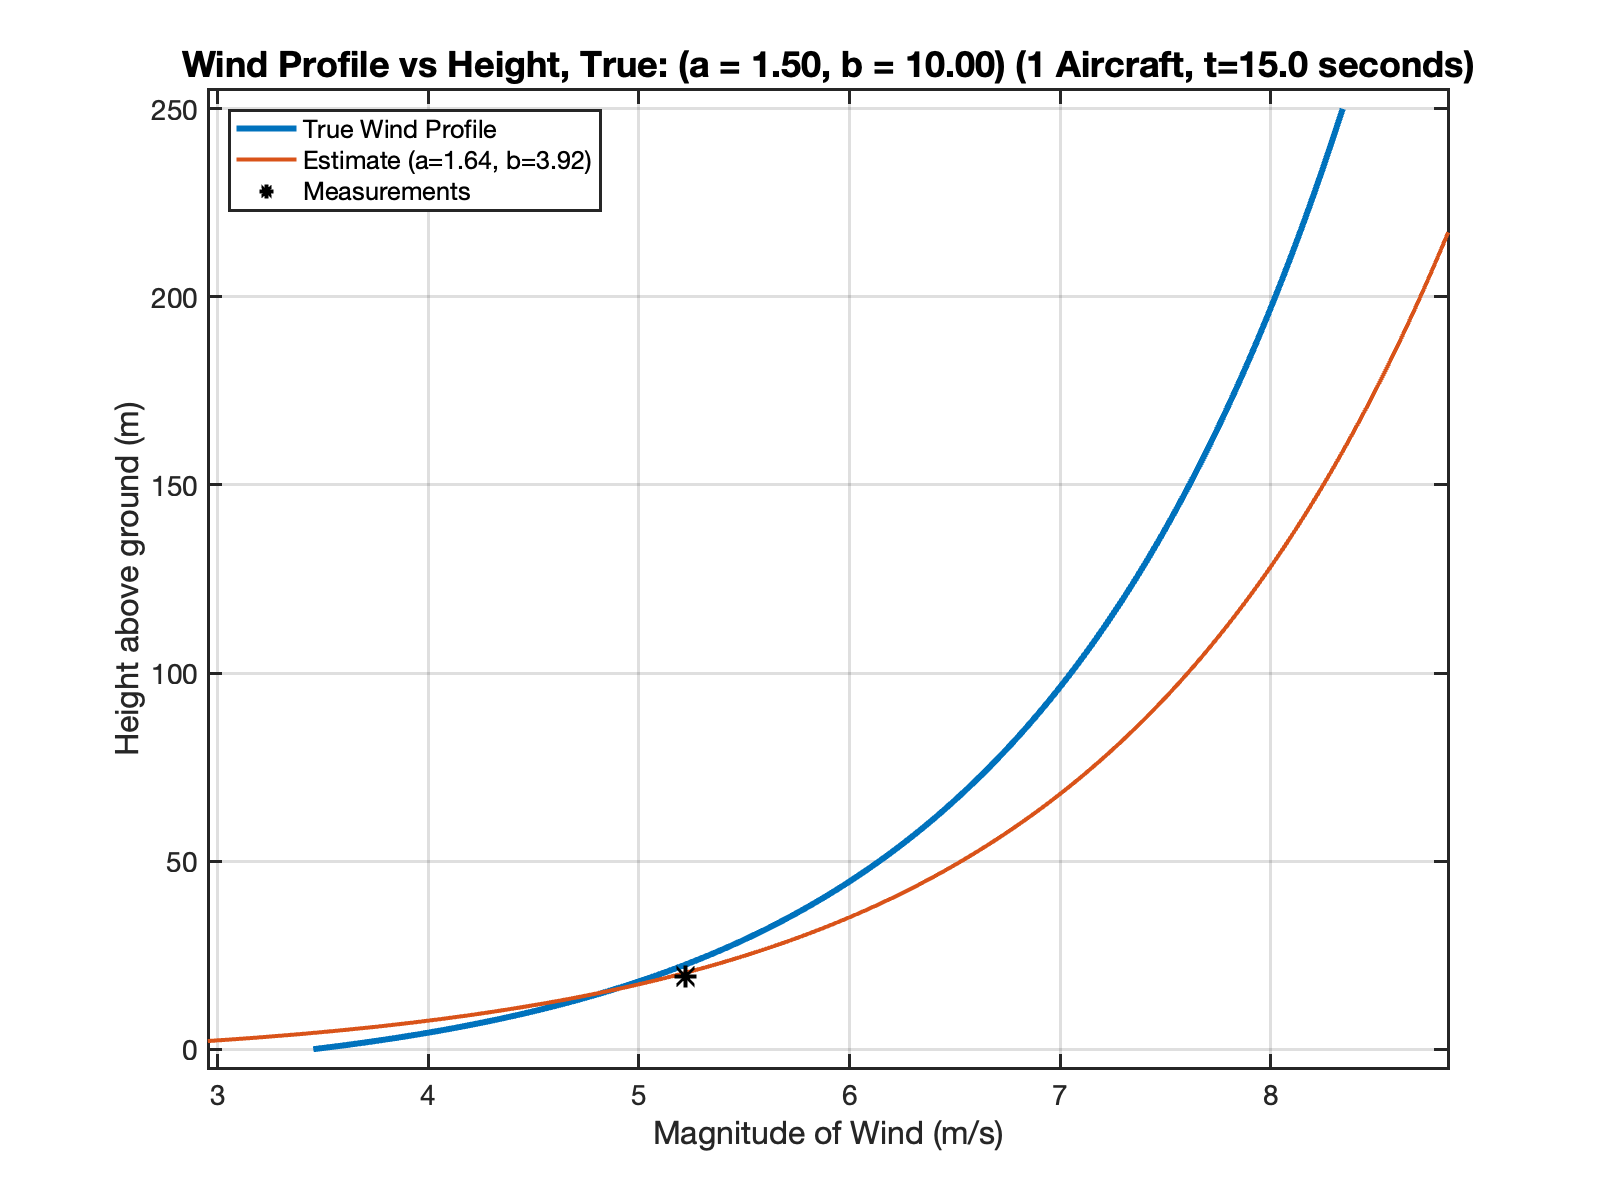
\includegraphics[width=0.5\textwidth]{images/single_15_sec.png}
    \caption{1 UAS, estimated wind gradient after 15 seconds into the simulation.}
    \label{fig:uas_traj_one_15}
\end{figure}

The results show the single UAS is able to correctly estimate its independent wind magnitude but not the entire gradient field.
By 15 seconds into the simulation, the UAS has a very accurate estimate of its own wind magnitude, as you can see the scatter point is almost exactly on the blue line showing the true wind. 
However, comparing 5 seconds vs 15 seconds, there is almost no improvement to the overall wind gradient estimation.
This is because the wind gradient the UAS has estimated is highly accurate to its singular measurement it knows.
This is the issue with only using a single UAS to estimate a wind gradient field; you only have a single observation point, which can lead to an inaccurate curve fit as there are infinite curves that could exist through that singular point.

A video showing the full simulation over 50 seconds for the single UAS case can be seen in the link at the top of the paper.

\subsection{Comparing Number of UAS}

To finalize the comparison and impact of using multiple UAS to estimate the wind gradient, we will compare the performance across a range of UAS.
Using a monte carlo simulation across 50 random wind gradient fields, with $a$ ranging from 1 to 5 and $b$ ranging from 1 to 25, we can average the difference between the true wind gradient and the estimated wind gradient for each number of UAS.
Each simulation will be ran for 50 seconds and the difference between the true and estimated gradient will be the average norm difference at the end of the simulation summed over all meter increments from 0 to 250 meters (eval the difference between true and estimated at each meter, up to 250).
Thus, 

\begin{equation}
    \text{Error} = \frac{1}{250} \sum_{h=0}^{250} \left\| \mathbf{g}_{true}(h) - \mathbf{g}_{est}(h) \right\|_2
\end{equation}

All UAS will be commanded to fly at a constant altitude guidance line in a stack formation of 25*(n) height above the ground.
Where n is the number of UAS, meaning all UAS will be spaced 25 meters apart, starting at a height of 25 meters off the ground.

The results for using 50 random wind gradient fields and averaging across all of them can be seen in Figure~\ref{fig:benchmark_num_uas}.

\begin{figure}[h]
    \centering
    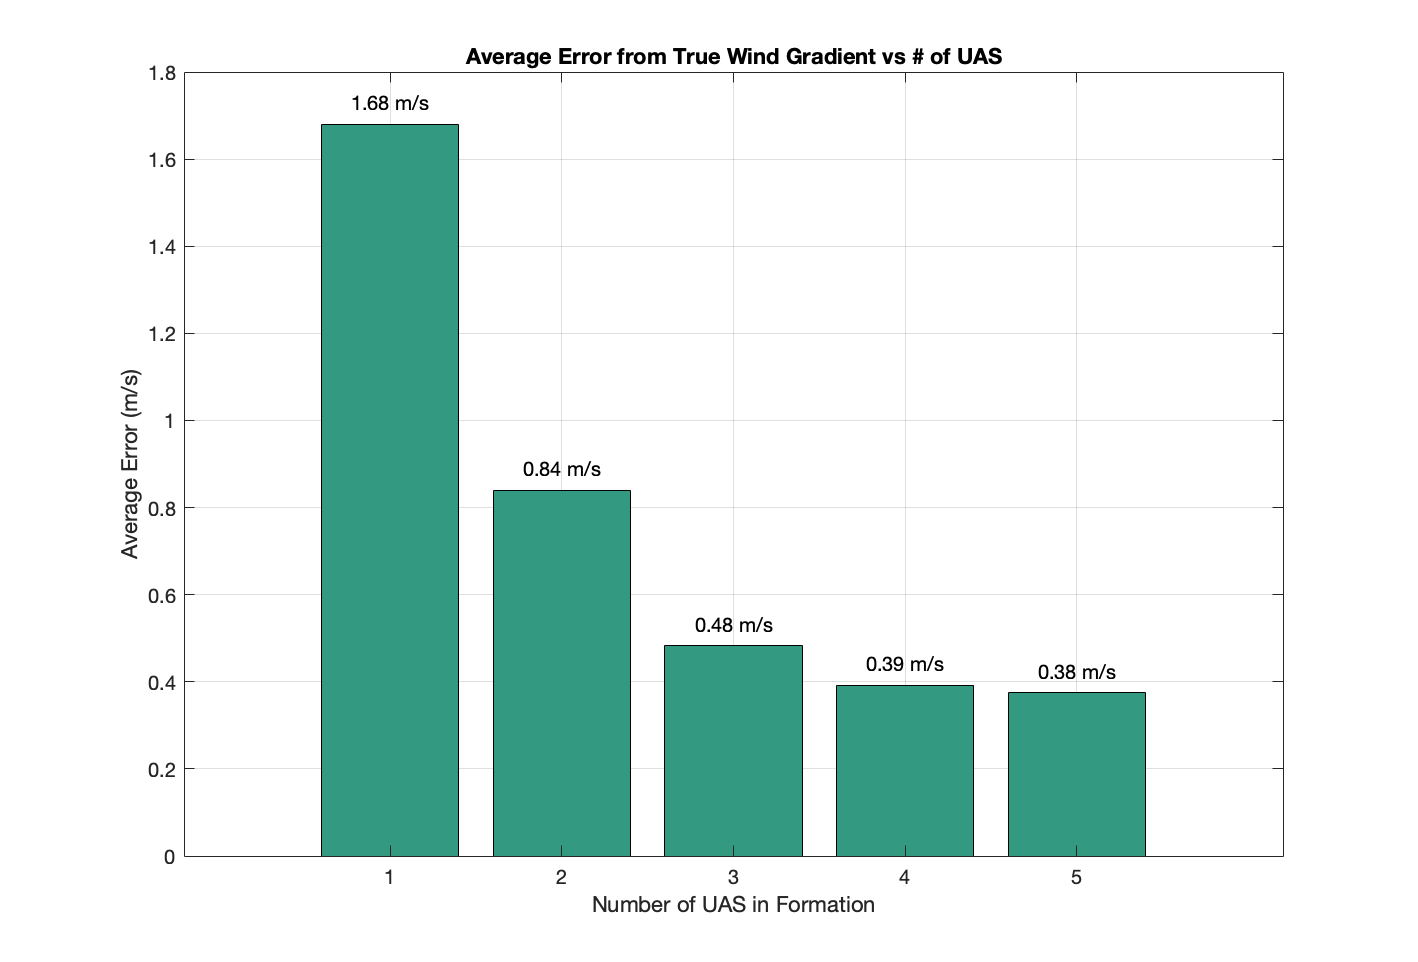
\includegraphics[width=0.5\textwidth]{images/bar_chart.png}
    \caption{Benchmarking the impact number of UAS has on estimating the wind gradient field.}
    \label{fig:benchmark_num_uas}
\end{figure}

Thus, the relationship is shown that as you increase the number of UAS flying in formation, working together to estimate the wind, the accuracy of the estimation increases.
This realtionship is quite obvious, but, its good to see the results confirm the relationship.
Its also important to see that the improvement to the estimation decreases as the number of UAS increases.
As you add more UAS, the improvement a invidiual UAS has to the overall estimation decreases. 
Therefore, depending on the application and accuracy needed in estimating the wind gradient, there is likely a sweet spot for the number of UAS to use.
Increasing the number of UAS used in a multi agent mission increases the cost and complexity of the mission and the benefits begins to decay as the number of UAS increases.


\subsection{Single UAS with a Climb Rate}

A final case we can consider is if a single UAS can accurately estimate the wind gradient if it is commanded to fly at a climb rate.
Instead of flying at a constant altitude, the UAS will be commanded to fly in a line that has a climb rate.
Specifically, we will command the UAS to follow a line specificed by the vector [1, 1, -0.5] in the inertial frame. 
Simulated over 50 seconds, the trajectory of the UAS can be seen in Figure~\ref{fig:uas_traj_one_climb}.

\begin{figure}[h]
    \centering
    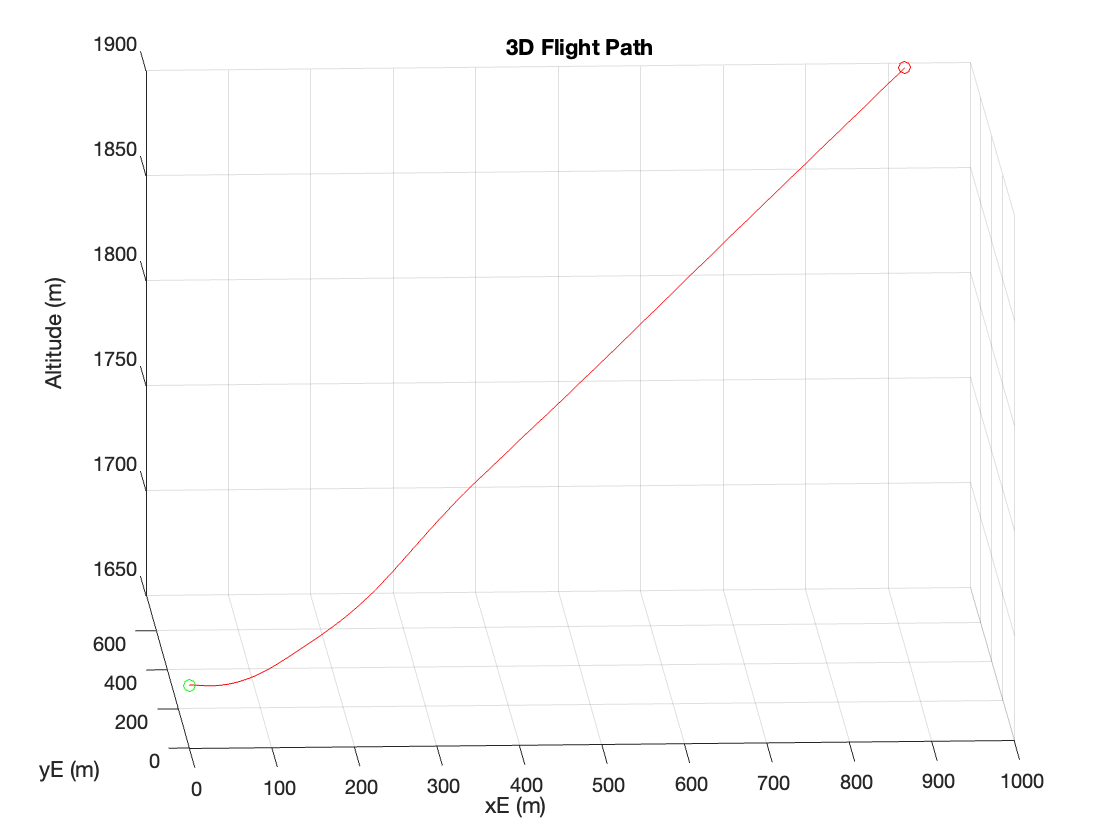
\includegraphics[width=0.5\textwidth]{images/3d_climb.png}
    \caption{3D Trajectory of a UAS following a line with a climb rate.}
    \label{fig:uas_traj_one_climb}
\end{figure}

The climb allows the UAS to traverse across the wind gradient, giving it more observability than just a single UAS flying at a constant altitude.

The results for the estimated wind gradient at 5 seconds, 20 seconds, and 40 seconds into the simulation can be seen in Figures~\ref{fig:uas_traj_one_climb_5}, ~\ref{fig:uas_traj_one_climb_20}, and ~\ref{fig:uas_traj_one_climb_40}, respectively.

\begin{figure}[h]
    \centering
    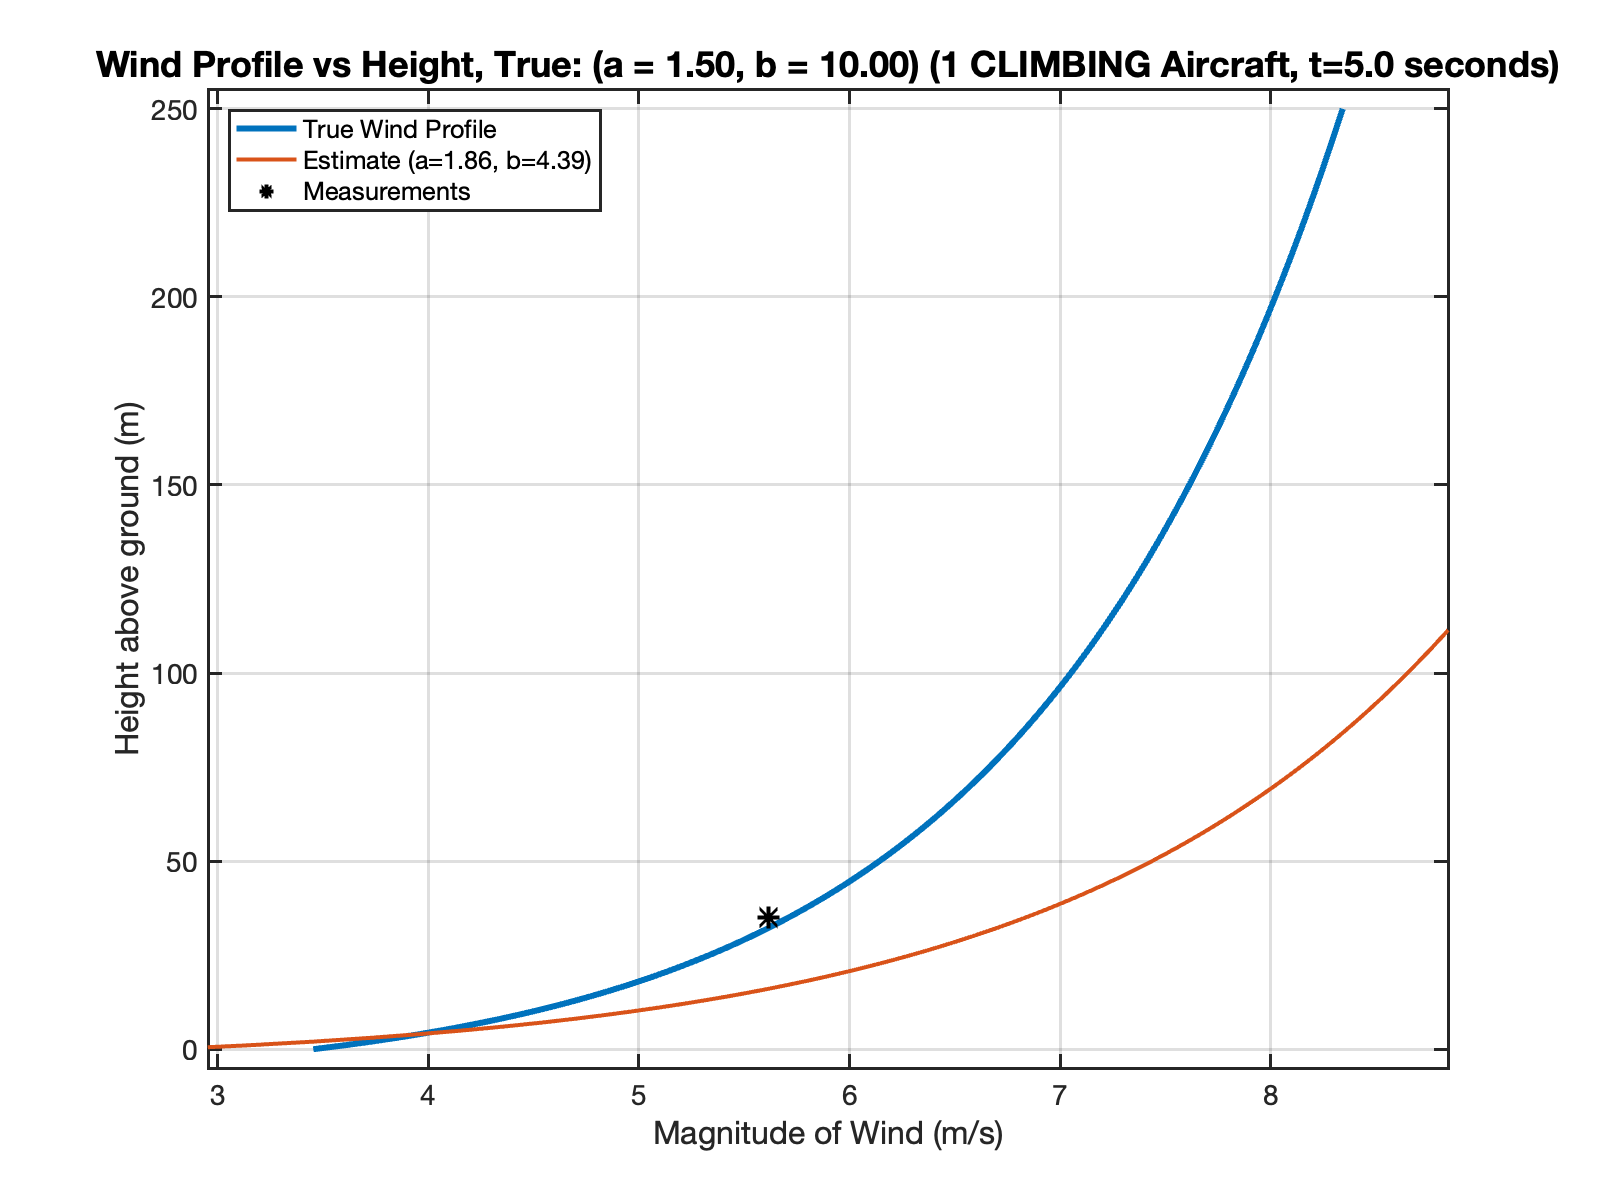
\includegraphics[width=0.5\textwidth]{images/climbing_5_sec.png}
    \caption{1 UAS, estimated wind gradient after 5 seconds into the simulation.}
    \label{fig:uas_traj_one_climb_5}
\end{figure}

\begin{figure}[h]
    \centering
    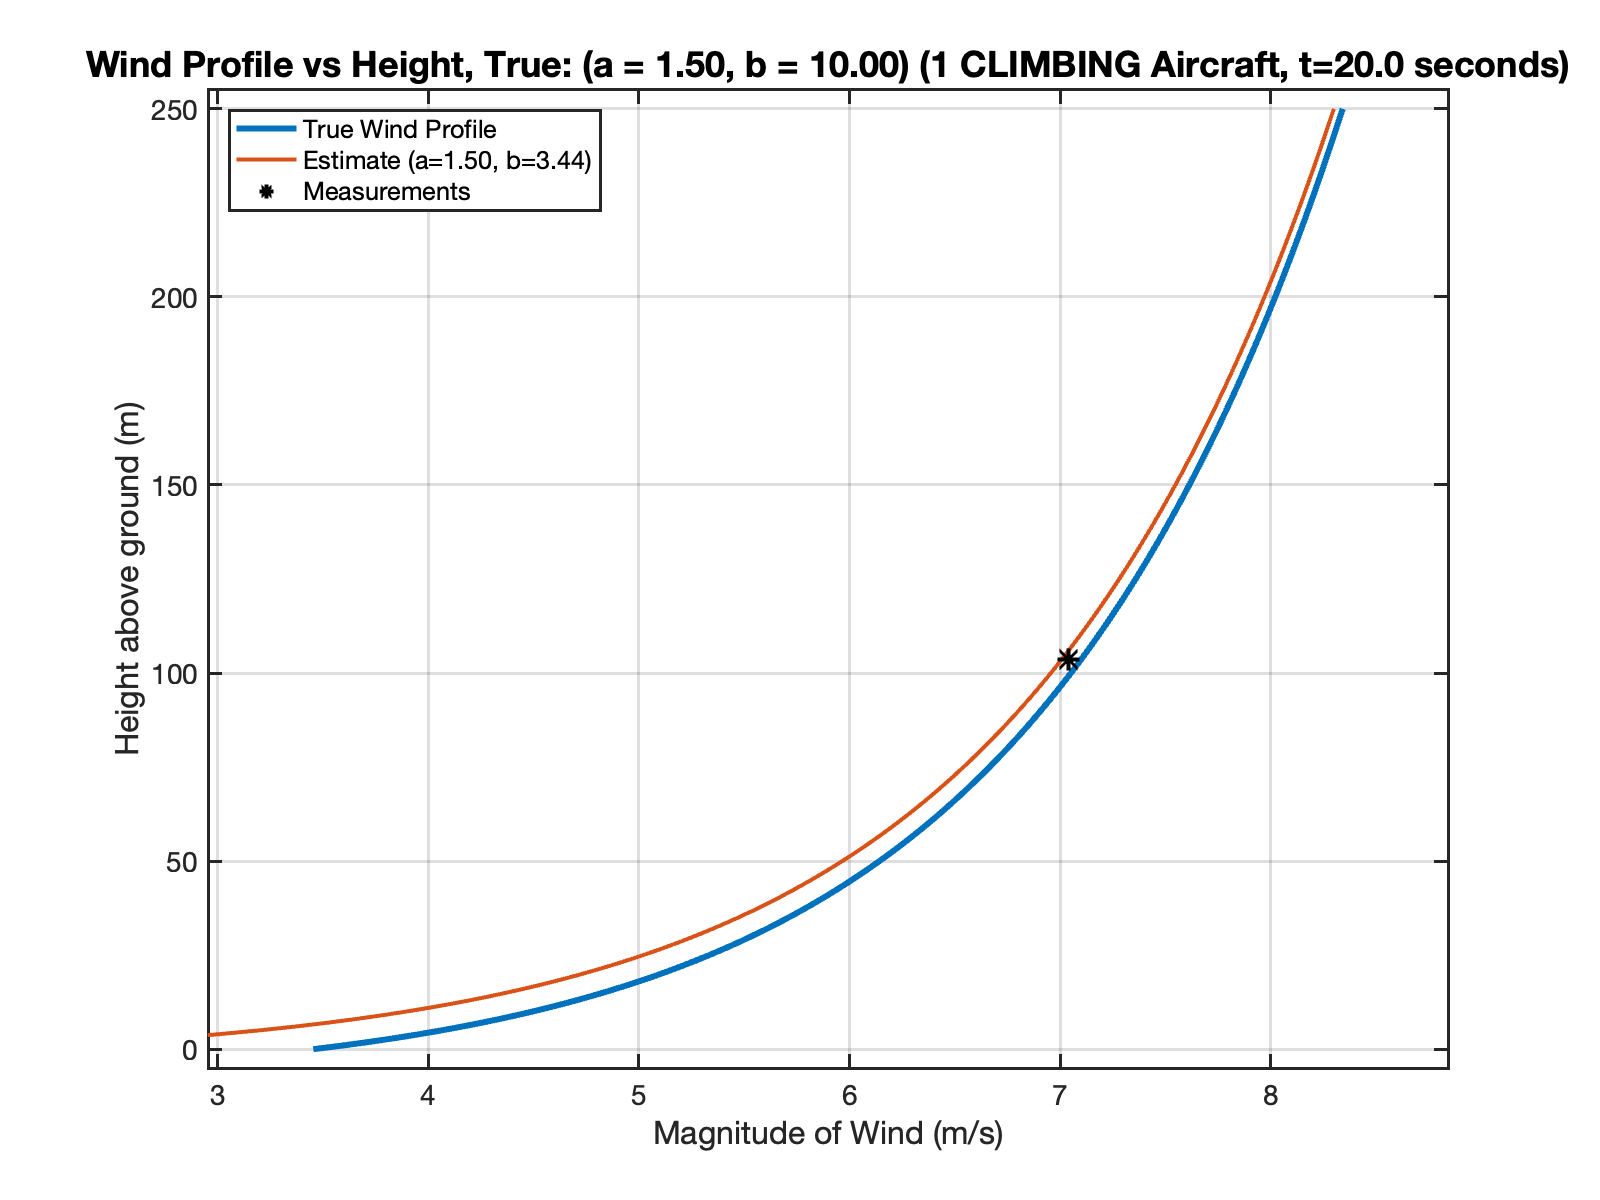
\includegraphics[width=0.5\textwidth]{images/climbing_20_sec.png}
    \caption{1 UAS, estimated wind gradient after 20 seconds into the simulation.}
    \label{fig:uas_traj_one_climb_20}
\end{figure}

\begin{figure}[h]
    \centering
    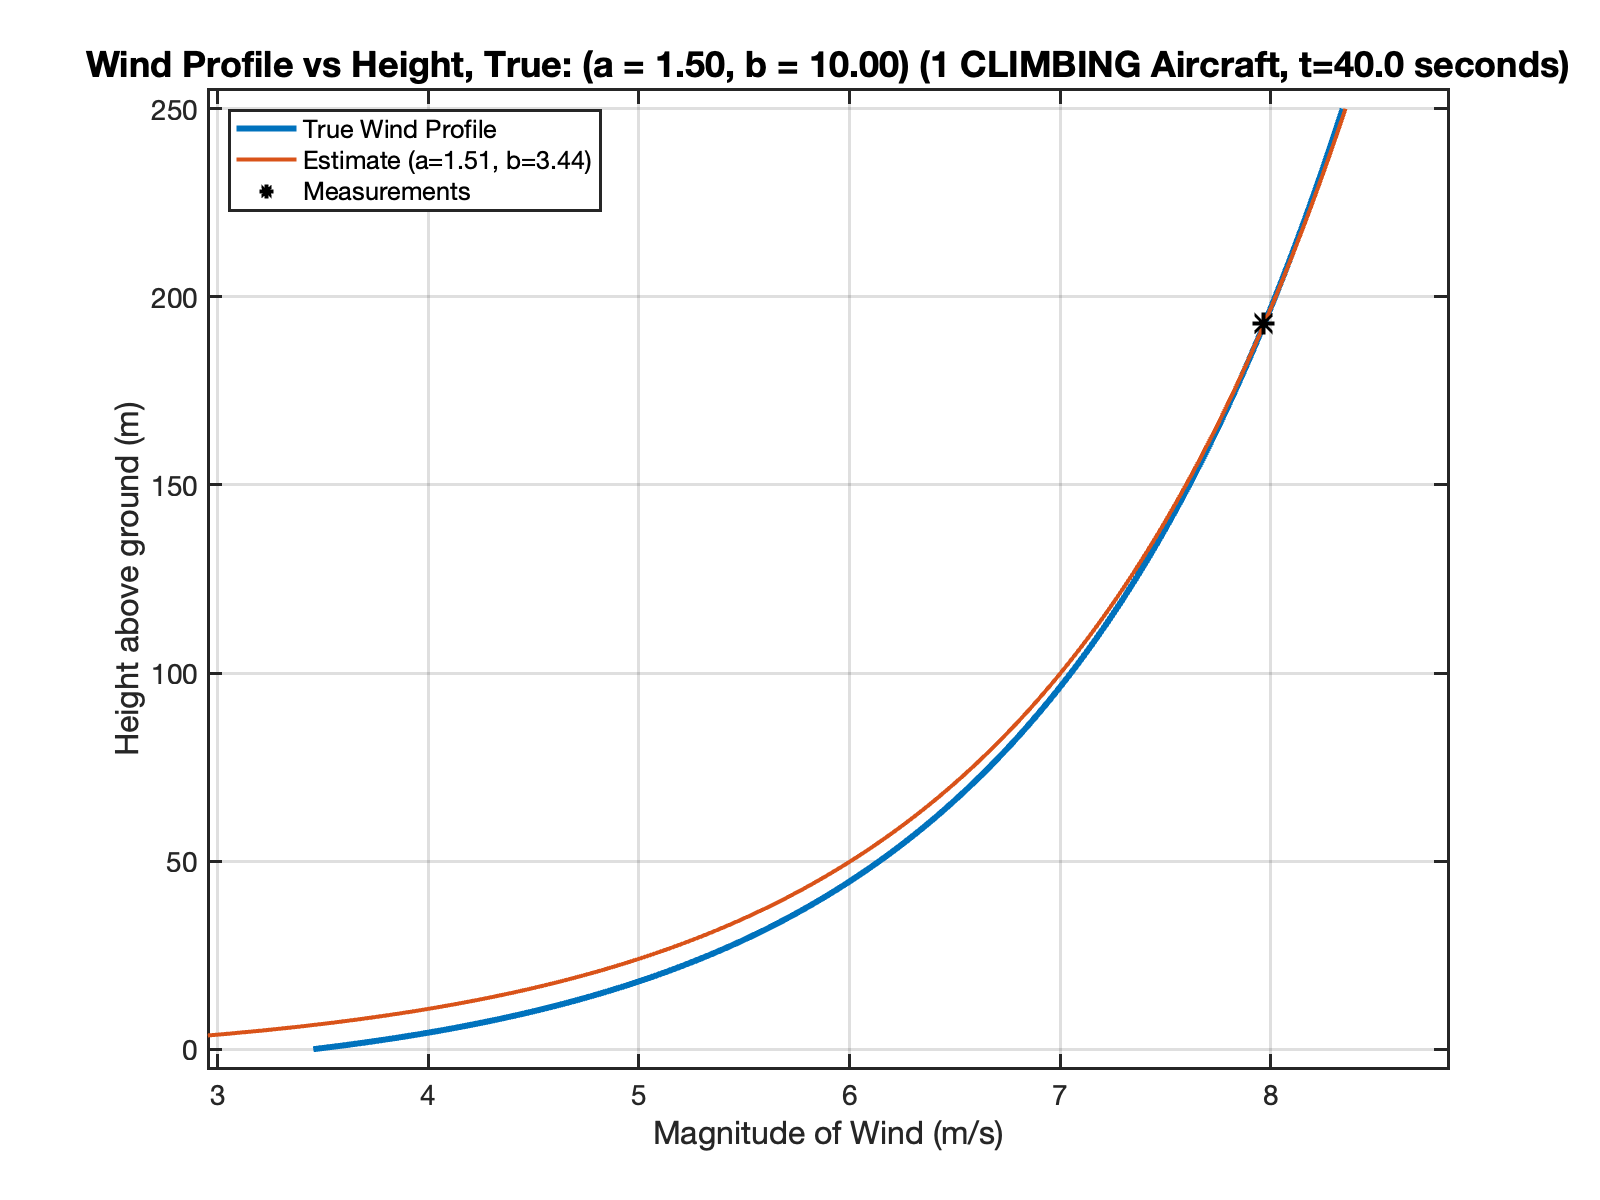
\includegraphics[width=0.5\textwidth]{images/climbing_40_sec.png}
    \caption{1 UAS, estimated wind gradient after 40 seconds into the simulation.}
    \label{fig:uas_traj_one_climb_40}
\end{figure}

As you can see from the figures, the single UAS is now able to more accurately estimate the wind gradient field, especially when compared against the constant height single UAS case seen in Figures~\ref{fig:uas_traj_one_5} and~\ref{fig:uas_traj_one_15}.
This makes sense as the issue a single UAS has is that it only has a single point of observation.
Thus, fitting a curve through that point is difficult as there are infinite solutions.
However, by commanding the UAS to climb, it is able to gain multiple observation points over time as it traverses the gradient.
This allows the online stochastic gradient descent algorithm to adjust to the entire profile of the gradient field.
The performance benefit of this is massive compared to the single, constant altitude, case shown above.
For a full video showing this scenario, see the link at the top of the paper.

One potential issue with this method of surveying the gradient field is that if the EKF is not able to accurately estimate the wind the entire algorithm, and potentially the autopilot, could fail.
The EKF for estimates wind by assuming the wind does not change over time, as discussed in the \textit{Adjusting the EKF} section.
Thus, by purposly climbing through a wind gradient, we are directly violating this assumption.
In this scenario, the EKF is still able to accurately estimate the wind at a given altitude, but, if the climb rate was higher or the gradient too big, the EKF could break and woudl not be able to estimate the wind.

Another potential issue with this scenario is that a single UAS may not be able to accurately estimate the wind gradient field if it begins changing over time.
This is a scenario we will not explore in this paper, we are always assuming a constant wind gradient, but, it is important to consider.
If the wind gradient changes over time, the single UAS, even with a climb rate, will still only have a single observation point in the time dimension.
The assumption that the single agent is able to survey the entire field over time, thus, increasing its observability, is not valid if the gradient is changing. 
The UAS may reach all altitudes in the gradient, but, the measurements may not be correlated to eachother if the gradient is changing.
However, a multi UAS formation could still accurately estimate the wind gradient as it instantanously has multiple obseveration points at any given time.


